%% ACMSE 2027 submission -- ACM sigconf, double-anonymous review.
%% Before submitting, compile inside the official ACMSE 2027 template package
%% (acmart-master-acmse2027-v0.1.zip) so its preset conference metadata is used.
\documentclass[sigconf,anonymous]{acmart}

\usepackage{booktabs}
\usepackage{multirow}
\usepackage{tikz}
\usetikzlibrary{arrows.meta, positioning, shapes.geometric, calc, fit, backgrounds}

\tikzset{
    party/.style={rectangle, rounded corners=2pt, draw=black!70,
                  fill=blue!5, align=center, minimum width=2.1cm,
                  minimum height=1.1cm, font=\small},
    server/.style={rectangle, rounded corners=2pt, draw=black!80,
                   fill=blue!15, align=center, minimum width=2.6cm,
                   minimum height=1.3cm, font=\small\bfseries},
    attacker/.style={rectangle, rounded corners=2pt, draw=red!60!black,
                     fill=red!8, align=center, minimum width=2.1cm,
                     minimum height=1.1cm, font=\small},
    flow/.style={-{Stealth[length=2.2mm]}, thick, black!80},
    leak/.style={-{Stealth[length=2.2mm]}, thick, red!60!black, dashed},
    sublabel/.style={font=\scriptsize, fill=white, inner sep=1pt}
}

%% Conference metadata (the official ACMSE 2027 template may already set these).
\setcopyright{acmlicensed}
\copyrightyear{2027}
\acmYear{2027}
\acmDOI{XXXXXXX.XXXXXXX}
\acmConference[ACMSE 2027]{2027 ACM Southeast Conference}{April 15--17, 2027}{Decatur, AL, USA}
\acmBooktitle{2027 ACM Southeast Conference (ACMSE 2027), April 15--17, 2027, Decatur, AL, USA}
\acmISBN{979-8-4007-2749-8}

\setlength{\emergencystretch}{2em}

\begin{document}

\title[Attribute Inference and Unlearning in VFL: Flower vs. SecretFlow]{Evaluating Attribute Inference Attacks in Vertical Federated Learning with Machine Unlearning: A Framework Comparison Between Flower and SecretFlow}

%% Author block is hidden by the "anonymous" option during review.
\author{Isaac Friedman}
\affiliation{%
  \institution{The University of Alabama}
  \city{Tuscaloosa}
  \state{Alabama}
  \country{USA}}
\email{ifriedman1@crimson.ua.edu}

\renewcommand{\shortauthors}{Friedman}

\begin{abstract}
Vertical Federated Learning (VFL) enables multiple clients to collaboratively train a model while keeping their features and attributes presumably private. Although raw data is never shared between clients, the intermediate representations that are exchanged during training can still contain information about the attributes that each client holds. This paper presents an end-to-end experimental framework that quantifies the attribute-inference risk of a two-party VFL system and tests whether machine unlearning can mitigate VFL's vulnerability to attribute inference. The framework is implemented twice, once on Flower and again on SecretFlow, both using a shared threat model and attack module. Baseline and unlearning experiments are run on the CelebA, MNIST, and NIH Chest X-ray14 datasets. We find that the attribute-inference attacker sits at or below random chance on the baseline model across all three datasets, with an attack success rate no higher than 0.50 and an AUC of approximately 0.50, and that gradient-ascent-based unlearning collapses task accuracy on MNIST and CelebA before it can meaningfully reduce the attack success rate. The Flower and SecretFlow runs produce identical metrics under matched conditions, showing that the framework layer is not an important variable for comparison.
\end{abstract}

\begin{CCSXML}
<ccs2012>
   <concept>
       <concept_id>10002978.10003029.10011150</concept_id>
       <concept_desc>Security and privacy~Privacy protections</concept_desc>
       <concept_significance>500</concept_significance>
       </concept>
   <concept>
       <concept_id>10010147.10010257</concept_id>
       <concept_desc>Computing methodologies~Machine learning</concept_desc>
       <concept_significance>300</concept_significance>
       </concept>
 </ccs2012>
\end{CCSXML}

\ccsdesc[500]{Security and privacy~Privacy protections}
\ccsdesc[300]{Computing methodologies~Machine learning}

\keywords{Vertical Federated Learning, Attribute Inference, Machine Unlearning, Flower, SecretFlow}

\maketitle

\section{Introduction}
Federated Learning (FL) removes the need to collect training data on a central server; instead, clients exchange model updates or intermediate representations while keeping the raw data on local machines. Vertical Federated Learning (VFL) is a feature-partitioned variant: different parties hold different \emph{columns} of the same records. A hospital might hold images while an insurer holds demographics; a photo service might hold an image while a separate service holds an attribute such as age or accessory. Only intermediate embeddings and gradients cross the network, allowing a model to be trained without the parties revealing their columns.

Despite this privacy-oriented design, VFL is not inherently private. Attribute inference attacks can recover the hidden columns of one client from the representations it (or the server) exposes during training. These attacks do not require access to raw data; they only need the embeddings that the collaboration produces. Machine unlearning offers a post-hoc knob: given a trained model and a ``forget set'', can we remove that set's influence without retraining from scratch? This paper asks: \emph{does machine unlearning reduce attribute-inference success in a VFL system, and does the result transfer across FL frameworks?}

We build a two-party VFL framework that is implemented twice, on Flower and on SecretFlow, under identical run conditions. We run baseline training and a gradient-ascent plus repair unlearning pass on three datasets that span data modalities and task types: MNIST (digits, balanced multiclass), CelebA (face attributes, with two labels available so one can be the target and the other the sensitive attribute), and NIH Chest X-ray14 (chest radiographs, imbalanced binary). Baseline and unlearning metrics are logged each epoch for direct comparison.

\section{Background and Related Work}

\paragraph{Vertical Federated Learning}
Horizontal FL distributes \emph{samples} across clients, while vertical FL distributes \emph{features}. In the VFL setting studied here, each party runs a local encoder over its columns and emits an embedding $z$, and a central server concatenates the per-party embeddings and trains a task head on the joint vector. Only $z$ (and the gradient flowing back to the local encoder during training) crosses the network. Liu et al.~\cite{liu2024vfl} provide a recent survey of the VFL literature, including the attack and defense taxonomy that frames the rest of this section.

\paragraph{Attribute Inference in Centralized Learning}
Yeom et al.~\cite{yeom2018privacy} tied membership and attribute inference risk directly to overfitting, showing that loss-based signals can separate members from non-members. Jia and Gong~\cite{jia2018attriguard} treated attribute inference as a practical adversarial problem and proposed AttriGuard, a defense that perturbs released data with adversarial examples. Song and Shmatikov~\cite{song2020overlearning} demonstrated overlearning: models trained for one task frequently encode sensitive attributes unrelated to that task in their internal representations, which is precisely the condition our VFL threat model assumes.

\paragraph{Inference Attacks Specific to VFL}
The VFL literature focuses on three attack groups. \emph{Label inference}, recovering the label a server or a party holds from gradient or embedding traces, was formalized by Fu et al.~\cite{fu2022label} and recently revisited by Liu et al.~\cite{liu2026revisiting}. \emph{Property and attribute inference} targets distributional or per-record properties of the non-attacker's columns; Bai et al.~\cite{bai2025provfl} propose ProVFL for this setting, and the attacker we build in this paper is a simplified per-record variant of this threat model. \emph{Reconstruction attacks} invert the embedding to an input estimate; Yao et al.~\cite{yao2025urvfl} give an undetectable reconstruction attack (URVFL) that motivates the use of embedding-only observations in our threat model. Monta\~{n}a-Fern\'{a}ndez and Ortega-Fernandez~\cite{montana2025gradient} study gradient-based inference attacks in federated learning more broadly, and Liu and Jiang~\cite{liu2025pgac} present PGAC, a general adversarial-attack framework for VFL specifically.

\paragraph{Defenses in VFL}
Defensive work complements the attack literature. Arazzi et al.~\cite{arazzi2025defense} propose a label-inference defense designed for VFL, and Madabushi et al.~\cite{madabushi2025privee} (PRIVEE) target feature-inference attacks at the representation layer. Both defenses operate \emph{at training time}: they change what the collaboration emits. They do not address the circumstance in which a record has already been trained on and its influence must be deleted. This is the setting that machine unlearning covers, which is why the present work pairs an unlearning pass with the attack evaluation.

\paragraph{Machine Unlearning}
Bourtoule et al.~\cite{bourtoule2021sisa} proposed SISA, a sharding-and-slicing training regime that lets a provider unlearn a data point by retraining only the affected shard. Xu et al.~\cite{xu2023survey} survey the broader family of exact and approximate unlearning methods and the trade-offs they make between speed, fidelity, and guarantees. Liu et al.~\cite{liu2021federated} extended these ideas to federated learning, where both the data and the model updates are distributed and where a ``forget'' request has to be honored without re-running the entire federation. The approach we evaluate here, gradient ascent on the forget set followed by retain-set repair, is an approximate, continuation-style form of unlearning as opposed to complete retraining.

\paragraph{Positioning of This Study}
This study does not propose a new attack or unlearning algorithm. Rather, it assembles an end-to-end VFL pipeline that measures attacker metrics with unlearning, implements it on two widely used frameworks (Flower and SecretFlow), and reports whether the attack-success story behaves the same way under both implementations. That cross-framework check, and specifically the pairing of VFL-native inference attacks~\cite{fu2022label,bai2025provfl,yao2025urvfl,liu2025pgac} with post-hoc unlearning~\cite{bourtoule2021sisa,liu2021federated}, addresses a current gap in VFL unlearning research.

\section{System Design}

The system is a two-client VFL setup. Client A holds image features (or the left half of a split image); Client B holds a sensitive attribute (on CelebA) or the right half of the image (on MNIST and NIH). Each client has a local encoder. During a training step, the encoders emit embeddings $z_A$ and $z_B$; these are concatenated and passed to a shared task head on the server. Gradients flow back so each client's encoder is updated from the task loss.

An external attacker observes $z_A$ only (never the raw image, never $z_B$, never the task label) and trains its own classifier to predict the sensitive attribute $a$ from $z_A$. This mirrors the honest-but-curious server threat model: the attacker sees everything that the collaboration already exposes, and nothing else.

The same Python modules (encoders, task head, loss, attacker, logging, and unlearning loop) are imported by both the Flower and SecretFlow runners through a few shared files (\texttt{common\_*.py}, \texttt{vfl\_unlearning.py}). Identical seeds and identical hyperparameters should therefore produce identical metrics on both sides, and any row-level disagreement would point at the framework layer rather than at the model.

Figure~\ref{fig:pipeline} shows the data flow. Clients A and B each encode their columns; the server concatenates the embeddings and trains the task head. The attacker sees only the embedding $z_A$ that Client A emits. After baseline training, the unlearning pass applies gradient ascent on a designated forget subset and then repairs on the retain subset.

\begin{figure*}[t]
\centering
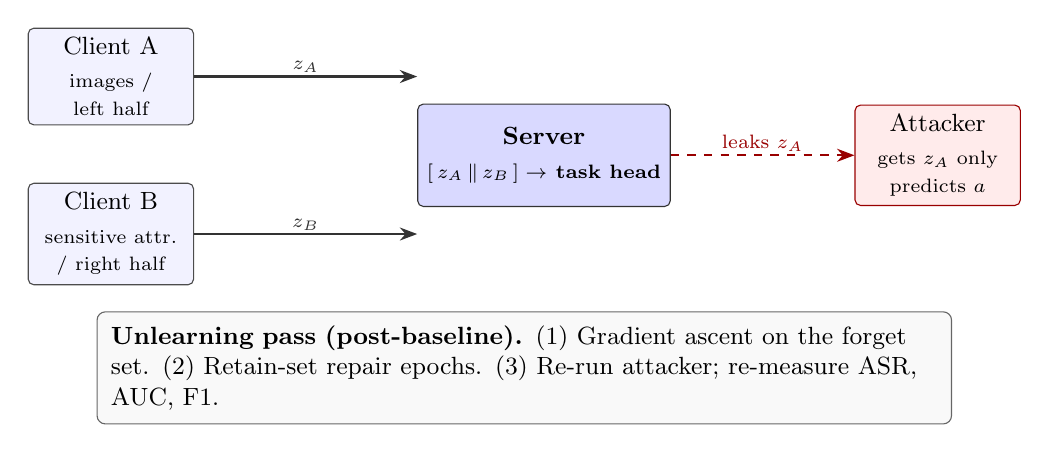
\begin{tikzpicture}[x=1cm, y=1cm]
    \node[party] (a) at (0, 1.0) {Client A\\[1pt]\scriptsize images /\\[-1pt]\scriptsize left half};
    \node[party] (b) at (0,-1.0) {Client B\\[1pt]\scriptsize sensitive attr.\\[-1pt]\scriptsize / right half};
    \node[server] (s) at (5.5, 0) {Server\\[1pt]\scriptsize $[\,z_A \,\Vert\, z_B\,] \rightarrow$ task head};
    \node[attacker] (atk) at (10.5, 0) {Attacker\\[1pt]\scriptsize gets $z_A$ only\\[-1pt]\scriptsize predicts $a$};
    \draw[flow] (a.east) -- node[sublabel, above]{$z_A$} (s.west |- a.east);
    \draw[flow] (b.east) -- node[sublabel, above]{$z_B$} (s.west |- b.east);
    \draw[leak] (s.east) -- node[sublabel, above]{leaks $z_A$} (atk.west);
    \node[rectangle, draw=black!60, rounded corners=3pt,
          fill=gray!5, text width=10.5cm, inner sep=5pt,
          align=left, font=\small] (unl) at (5.25,-2.7) {
      \textbf{Unlearning pass (post-baseline).}
      (1)~Gradient ascent on the forget set.
      (2)~Retain-set repair epochs.
      (3)~Re-run attacker; re-measure ASR, AUC, F1.
    };
\end{tikzpicture}
\caption{Two-Client VFL Pipeline}
\Description{Block diagram. Client A and Client B send embeddings z_A and z_B to a server, which concatenates them and trains a task head. A dashed arrow shows z_A leaking from the server to an attacker that predicts the sensitive attribute. A box below describes the unlearning pass: gradient ascent on the forget set, retain-set repair, then re-running the attacker.}
\label{fig:pipeline}
\end{figure*}

\section{Methodology}

\paragraph{Datasets and Tasks}
Three datasets are used, each illustrating a different modality and label structure. On MNIST the images are split vertically (28$\times$14 pixels per party) and the task is standard 10-way digit classification. On CelebA the images are held by Client A and an attribute is held by Client B; \texttt{Smiling} is the task label and \texttt{Eyeglasses} is the sensitive attribute the attacker tries to recover. On NIH Chest X-ray14 the images are again split vertically between the parties and the task is binary \texttt{Infiltration} (present vs.\ absent), which is highly class-imbalanced.

\paragraph{Models}
Party encoders are lightweight convolutional stacks that emit a fixed-width embedding per party. The server head is a small MLP that consumes the concatenated embeddings. The attacker is a separate MLP trained on $z_A$ alone with the sensitive attribute as its label. All model definitions live in \texttt{common\_*\_vfl.py} and are shared by the Flower and SecretFlow run scripts.

\paragraph{Baseline Phase}
The joint model is trained end-to-end for a fixed number of epochs (three on MNIST and CelebA, two on NIH) using Adam and cross-entropy. We log per-epoch train/test loss and accuracy and, after each epoch, evaluate the attacker on $z_A$ to obtain the attack accuracy (attack success rate, ASR), attack AUC, and attack F1.

\paragraph{Unlearning Phase}
At the end of baseline training the training set is split into a \emph{forget} subset (10\% of training rows, seed-controlled) and a \emph{retain} subset (the remaining 90\%). One epoch of \emph{gradient ascent} is applied on the forget set, in which the sign of the task loss is flipped so that the encoders and head actively drift away from the forget-set predictions. This is followed by one epoch of repair on the retain set with the ordinary loss. The attacker is re-evaluated on $z_A$ at the end of the unlearning pass.

\paragraph{Metrics and Deltas}
For every run we log a \texttt{metrics.csv} file with one row per epoch and a phase tag (\texttt{baseline} or \texttt{unlearn}), and append one row to \texttt{run\_summary.csv} that carries the final baseline values, the final post-unlearning values, and their signed deltas for each of 14 metrics, so that pre- and post-unlearning comparisons can be read without re-parsing the per-epoch file.

\section{Experimental Setup}

All runners are implemented in PyTorch 2.3 and share pinned dependencies (\texttt{torch==2.3.1}, \texttt{torchvision==0.18.1}, \texttt{pandas==2.2.2}, \texttt{scikit-learn==1.4.2}, \texttt{numpy==1.26.4}, \texttt{Pillow==10.3.0}). Each framework has its own virtual environment built from a per-framework \texttt{requirements.txt}. A PowerShell bootstrap script builds both environments, and a smoke-test script drives a one-epoch pass through every framework and dataset pair and verifies that the expected columns are present.

Runs reported here use Adam with lightweight hyperparameters tuned per dataset, batch size 128, seed~7, a forget fraction of 0.10, one unlearning epoch, and one repair epoch. All runs were executed on a local CPU for reproducibility and to make the Flower and SecretFlow runs directly comparable; the code also supports CUDA.

\section{Results}

\subsection{Baseline per Dataset}

Table~\ref{tab:baseline} shows the per-epoch baseline metrics recorded by the Flower runner on each dataset. Each row is copied from \texttt{metrics.csv}; only floating-point precision and column selection have been adjusted for presentation, and accuracy columns are in $[0,1]$. The MNIST task is 10-class digit classification on vertically split images; the CelebA task is \texttt{Smiling}, with \texttt{Eyeglasses} held by Client B as the sensitive attribute; and the NIH task is binary \texttt{Infiltration}, for which two baseline epochs were run.

\begin{table*}[t]
\centering
\small
\caption{Flower Baseline Metrics per Dataset}
\label{tab:baseline}
\begin{tabular}{@{}llcccccc@{}}
\toprule
Dataset & Epoch & Train loss & Train acc & Test acc & ASR & AUC & F1 \\
\midrule
\multirow{3}{*}{MNIST}
    & 1 & 0.805 & 0.729 & 0.731 & 0.456 & 0.492 & 0.479 \\
    & 2 & 0.501 & 0.838 & 0.848 & 0.430 & 0.486 & 0.492 \\
    & 3 & 0.335 & 0.897 & 0.903 & 0.421 & 0.483 & 0.505 \\
\addlinespace[2pt]
\multirow{3}{*}{CelebA}
    & 1 & 0.630 & 0.648 & 0.633 & 0.499 & 0.513 & 0.512 \\
    & 2 & 0.524 & 0.740 & 0.733 & 0.492 & 0.503 & 0.534 \\
    & 3 & 0.471 & 0.778 & 0.768 & 0.487 & 0.500 & 0.539 \\
\addlinespace[2pt]
\multirow{2}{*}{NIH Chest X-ray14}
    & 1 & 0.461 & 0.823 & 0.823 & 0.362 & 0.500 & 0.424 \\
    & 2 & 0.461 & 0.823 & 0.823 & 0.362 & 0.500 & 0.424 \\
\bottomrule
\end{tabular}
\end{table*}

Two patterns stand out in Table~\ref{tab:baseline}. First, the joint VFL model learns each task: train and test accuracy rise over the three baseline epochs on MNIST (0.73 $\rightarrow$ 0.90 test) and CelebA (0.63 $\rightarrow$ 0.77 test), while NIH is pinned at $\approx 0.82$ test accuracy by the majority class. Second, the attacker never gains a meaningful signal from the embedding $z_A$ in these runs: ASR stays in $[0.36,\,0.50]$ and AUC sits at $\approx 0.50$ on all three datasets. In other words, the baseline attacker is at or below random chance.

\subsection{Framework Parity: Flower vs. SecretFlow}

Table~\ref{tab:parity} pairs the final-epoch numbers from the Flower and SecretFlow runners on matched MNIST and CelebA runs, for both the baseline and unlearning phases. Because both runners import the same model, loss, and attacker code and receive identical seeds, the rows are identical.

\begin{table}[t]
\centering
\small
\caption{Flower vs. SecretFlow Final-Epoch Metrics}
\label{tab:parity}
\begin{tabular}{@{}llcccc@{}}
\toprule
Run & Framework & Test acc & ASR & AUC & F1 \\
\midrule
\multirow{2}{*}{MNIST baseline}
    & Flower     & 0.903 & 0.421 & 0.483 & 0.505 \\
    & SecretFlow & 0.903 & 0.421 & 0.483 & 0.505 \\
\addlinespace[2pt]
\multirow{2}{*}{MNIST unlearn}
    & Flower     & 0.318 & 0.437 & 0.486 & 0.484 \\
    & SecretFlow & 0.318 & 0.437 & 0.486 & 0.484 \\
\addlinespace[2pt]
\multirow{2}{*}{CelebA baseline}
    & Flower     & 0.768 & 0.487 & 0.500 & 0.539 \\
    & SecretFlow & 0.768 & 0.487 & 0.500 & 0.539 \\
\addlinespace[2pt]
\multirow{2}{*}{CelebA unlearn}
    & Flower     & 0.506 & 0.488 & 0.487 & 0.472 \\
    & SecretFlow & 0.506 & 0.488 & 0.487 & 0.472 \\
\bottomrule
\end{tabular}
\end{table}

Framework-induced variance is therefore effectively zero in the current design. Any future difference between Flower and SecretFlow in these metrics would have to originate in the communication layer (e.g., gradient serialization or aggregation) rather than in the model or attacker code.

\subsection{Baseline to Unlearning Delta}

Table~\ref{tab:delta} pairs the last baseline-epoch row with the post-unlearning row for MNIST and CelebA. Test, Retain, and Forget are task accuracies on the test, retain, and forget sets. Baseline values are from the last baseline epoch; unlearning values are logged after one gradient-ascent epoch plus one repair epoch. The NIH run completed only the baseline phase, so NIH is reported in Table~\ref{tab:baseline} only.

\begin{table}[t]
\centering
\footnotesize
\setlength{\tabcolsep}{3pt}
\caption{Pre- and Post-Unlearning Comparison}
\label{tab:delta}
\begin{tabular}{@{}lccccccc@{}}
\toprule
Dataset & Phase & Test & Retain & Forget & ASR & AUC & F1 \\
\midrule
\multirow{2}{*}{MNIST}
    & baseline & 0.903 & 0.898 & 0.894 & 0.421 & 0.483 & 0.505 \\
    & unlearn  & 0.318 & 0.313 & 0.297 & 0.437 & 0.486 & 0.484 \\
\addlinespace[2pt]
\multirow{2}{*}{CelebA}
    & baseline & 0.768 & 0.779 & 0.775 & 0.487 & 0.500 & 0.539 \\
    & unlearn  & 0.506 & 0.485 & 0.483 & 0.488 & 0.487 & 0.472 \\
\bottomrule
\end{tabular}
\end{table}

Three observations follow directly from the numbers.

\emph{(1) Task accuracy is the pressure point.} On MNIST the single unlearning epoch drops test accuracy from 0.90 to 0.32 and retain accuracy from 0.90 to 0.31. On CelebA it drops test accuracy from 0.77 to 0.51. These are not small perturbations; they indicate that the gradient-ascent step at our current learning rate badly overshoots and that one repair epoch is not enough to walk the model back. A defense that halves test accuracy to shift ASR by one point is not worth deploying.

\emph{(2) ASR and AUC barely move.} The attacker's success is numerically indistinguishable from the baseline: MNIST ASR $0.421 \rightarrow 0.437$, CelebA ASR $0.487 \rightarrow 0.488$. The near-chance baseline from the previous subsection is the dominating factor here. When the attacker is already at 0.5 on a binary attribute, there is almost nothing for unlearning to shrink.

\emph{(3) F1 confirms the reading.} Attacker F1 on both MNIST and CelebA sits in the 0.47--0.54 band both before and after unlearning. Because F1 is the harmonic mean of the attacker's precision and recall, that band indicates the attacker is producing roughly balanced predictions around chance rather than concentrating on one class, which is consistent with the AUC $\approx 0.50$ signal.

\section{Discussion}

The clearest message in the results is that this experiment's attacker is too weak to expose a difference that the unlearning process could reasonably shrink. An attacker at chance combined with aggressive unlearning is a poor pairing: a reduction in ASR can only be observed if ASR was non-trivial to begin with. The next iteration should therefore start from a stronger baseline attacker, either a deeper MLP head on $z_A$ or a shadow-model-style membership inference attack that learns a member/non-member split from per-sample loss statistics, before applying the unlearning process.

The framework-parity result is a positive null. Because Flower and SecretFlow produced identical rows under matched seeds, the framework layer is not a source of variance in this design. That is the setup needed to later distinguish communication-layer behavior from model behavior. The comparison between the two frameworks in this paper is therefore a procedural comparison: both frameworks can host the same VFL pipeline and the same attack, and the experimental setup is ready to catch framework-specific effects once they are introduced.

The unlearning results call for a hyperparameter sweep more than a new algorithm. Task accuracy collapses because one gradient-ascent epoch at the baseline learning rate moves the model too far, and one repair epoch is not enough to bring it back. A smaller ascent learning rate, more repair epochs, or a smaller forget fraction are all adjustments worth pursuing before concluding that gradient-ascent unlearning is ineffective in this setting.

\section{Future Work}

The immediate next step is to complete an end-to-end run of the baseline and unlearning loop on the NIH dataset, so that it has both a pre- and post-unlearning row. A hyperparameter sweep on the unlearning step would follow, varying the forget learning rate and the number of repair epochs to find the point at which test accuracy is preserved. In parallel, the code base, including the pinned requirements and the bootstrap and smoke-test scripts, is being prepared for public release.

Beyond these runs, two follow-ups are natural. First, a stronger baseline attacker, either a deeper inference head or a shadow-model membership attack, would create a non-trivial ASR to measure against. Second, the per-framework virtual environments are already isolated, which makes it easy to add a third framework and ask the same parity question; secure multi-party computation backends (e.g., SecretFlow's SPU) are the most interesting candidate because any divergence from the CPU/PyTorch rows would be traceable to the cryptographic layer rather than the model. It would also be valuable to vary other factors, such as adding more clients, mounting attacks from other positions such as the server, or using a larger set of datasets.

\section{Conclusion}

This study built a two-client VFL framework, implemented it on Flower and SecretFlow through a shared model and attacker module, and evaluated attribute-inference risk with and without a gradient-ascent unlearning pass on MNIST, CelebA, and NIH Chest X-ray14. The framework layer disappears as a source of variance: Flower and SecretFlow produce identical metrics under matched seeds. The attacker is already at or near chance on the baseline, and the current gradient-ascent unlearning step lowers task accuracy far more than it affects attack success.

%% Acknowledgments are hidden automatically by the "anonymous" option.
%% Uncomment for the camera-ready version if desired.
% \begin{acks}
% The author thanks Prof. Sayanton Dibbo for guidance on this project.
% \end{acks}

\bibliographystyle{ACM-Reference-Format}
\bibliography{references}

\end{document}
